
\section{Architecture} 
\label {chapter:architecture}
\begin{itemize}
\item 1. How many input neurons are needed for this assignment?\\
Ten, as there are ten initial inputs (features). The network should classify 10 features into 7 classes.
\item 2. How many output neurons do you require?\\
As was described above the network goes from 10 features (inputs) to 7 classes (outputs), so there are 7 output neurons.
\item 3. How many hidden neurons will your network have?\\
The amount of hidden neurons is not fixed. It depends on a lot of different factors and it is almost impossible to tell the optimum amount. We started testing with 10 hidden neurons per layer, but eventually settled on 50 neurons per layer wich provided the best result.
\item 4. Which activation function(s) will you use?\\
We will use the Sigmoid activation function.
\item 5. Give a schematic diagram of your complete network\\
This schematic only has one hidden layer, ours has multiple but the setup is the same. Also included in the image is a schematic that shows how a neuron handles inputs to create an output.
(using the sigmoid activation function).
\end{itemize}

\begin{figure}[!h]
\begin{center}
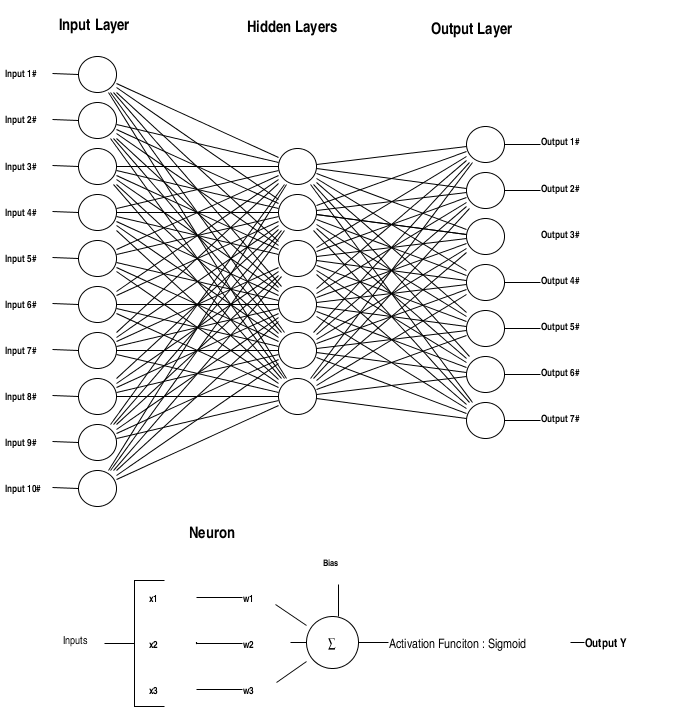
\includegraphics[width=11cm]{images/schemeit-project.png}
\caption{Schematic }
\label{schematic}
\end{center}
\end{figure}
\FloatBarrier

